% !TeX program = pdflatex
% !TeX encoding = UTF-8
\documentclass[fontsize=11pt, parskip=half]{scrartcl}

%preamble loading packages and so on

%packages
\usepackage{scrlayer-scrpage}
\usepackage[datesep={.}, style=ddmmyyyy]{datetime2}
\usepackage{graphicx}
\usepackage{multicol}
\usepackage[colorlinks=true, urlcolor=blue, linkcolor=black]{hyperref}
\usepackage{amsmath}
\usepackage{mathtools}
\usepackage{listings}
\usepackage{csquotes}
\usepackage{wrapfig}
\usepackage{caption}
\usepackage[a4paper, top=2cm, bottom=2cm, left=2cm, right=2cm]{geometry}
\MakeOuterQuote{"}
\usepackage{array}   % for \newcolumntype macro
\usepackage{multirow}
\newcolumntype{L}{>{$}l<{$}} % math-mode version of "l" column type
\newcolumntype{C}{>{$}c<{$}} % math-mode version of "c" column type
\newcolumntype{R}{>{$}r<{$}} % math-mode version of "r" column type

%%%%%%%%%%%%%%
%commands
%%%%%%%%%%%%%%

%formatting
\renewcommand{\thesubsection}{\thesection.H\arabic{subsection}} %changes subsection labelling to alphabetical -> 1.a instead of 1.1
\captionsetup{labelfont=bf, textfont=it, justification=raggedright,singlelinecheck=false, justification=centering}
%generalmath
\newcommand\br[1]{\ensuremath{\left(#1\right)}}
\newcommand\modulo[1]{\ensuremath{\bmod{\left(#1\right)}}} %adds \modulo{} as command for modulo calculations. Content is placed in brackets.
\DeclarePairedDelimiter\ceil{\lceil}{\rceil} %defines \ceil{} as command producing mathematical ceiling symbols around content
\DeclarePairedDelimiter\floor{\lfloor}{\rfloor} %defines \floor{} as command producing mathematical floor symbols around content
\newcommand\bsum[3]{\ensuremath{\sum_{#1}^{#2}{\left({#3}\right)}}} %defines \bsum{}{}{} as command for large sum with start, end and content. Content is placed in brackets.
\newcommand\bprod[3]{\ensuremath{\prod_{#1}^{#2}{\left({#3}\right)}}} %defines \bprod{}{}{} as command for large product with start, end and content. Content is placed in brackets.
\newcommand\texeq[1]{\stackrel{\mathclap{\normalfont\mbox{\scriptsize {#1}}}}{=}} %defines \teq as command for equal sign with subscript
\newcommand\defeq{\ensuremath{=_{def}}} %defines \defeq as command for definition with equal sign

%formal logic
\newcommand\bland[3]{\ensuremath{\bigwedge_{#1}^{#2}{\left({#3}\right)}}} %defines \bland{}{}{} as command for large logical AND with start, end and content. Content is placed in brackets.
\newcommand\blor[3]{\ensuremath{\bigvee_{#1}^{#2}{\left({#3}\right)}}} %defines \bland{}{}{} as command for large logical OR with start, end and content. Content is placed in brackets.
\newcommand\bforall[2]{\ensuremath{\left(\forall {#1}\right) \left[{#2}\right]}} %defines \bforall{}{} as command for logical forall with variable and content. forall and variable are placed within (), Content is placed in [].
\newcommand\bexists[2]{\ensuremath{\left(\exists {#1}\right) \left[{#2}\right]}} %defines \bexists{}{} as command for logical exists with variable and content. forall and variable are placed within (), Content is placed in [].

%Mathmatical Sets (Mengenlehre)
\newcommand\intenset[2]{\ensuremath{\left\lbrace {#1} \mid {#2} \right\rbrace}} %defines \intenset{}{} as command for intensional notation of mathmatical sets: {@|@}.
\newcommand\intensetU[2]{\ensuremath{\left\lbrace {#1} \in U \mid {#2} \right\rbrace}} %defines \intensetU{}{} as command for intensional notation of mathmatical sets: {@ \in U |@}.
\newcommand\extenset[1]{\ensuremath{\left\lbrace {#1} \right\rbrace}} %defines \extenset{} as command for extensional notation of mathmatical sets: {@}.

% referencing
\newcommand\fref[1]{\textbf{Figure \ref{#1}}} % defines \fref{} as command printing "Figure figurenumber" in bold.

%Title, Author, ...
\makeatletter
\title{Conspiracy narratives and public perception of 15-minute cities on YouTube}\let\Title\@title
\def \papersubtitle {Project Report}
\def \paperdeadline {21.08.2024}
% seminar information
\def \paperevaluator {Max Pellert}
\def \paperseminar {Social Media Data Analysis}
\def \papersemester {Summer/Winter Semester 2024}
\def \paperdepartment {Department of Politics and Public Administration}
\def \paperuniversity {University of Konstanz}
% personal information
\def \paperemail {julia.king@uni-konstanz.de}
\def \paperprogramme {M.Sc. Social and Economic Data Science}
\def \papermatriculationnr {01/911139}
\author{Julia King}          \let\Author\@author
\date{\today}           \let\Date\@date
\makeatother

% Page Layout
\ihead{Julia K.}
\chead{Conspiracy narratives \& public perception of 15-minute cities on YouTube}
\ohead{SMDA}

% caption setup
\captionsetup{labelfont=bf, textfont=it, justification=raggedright,singlelinecheck=false}

% citation setup
\usepackage[style=apa, sorting=nyt, backend=biber]{biblatex}
\usepackage{etoolbox} % If not already included
\addbibresource{citations.bib} %bibliography file

\begin{document}
\setlength{\columnsep}{25pt}

% Title Page, do not change here, variables are defined above!
\begin{titlepage}
    \newcommand{\HRule}{\rule{\linewidth}{0.5mm}}
    
    \begin{flushleft} % Upper left corner
        \large
        \paperuniversity\\
        \paperdepartment\\
        \papersemester\\
        \paperseminar\\
        \paperevaluator
    \end{flushleft}
    
    \vfill
    
    \begin{center} % Centered title and date
        \huge\bfseries \Title\\
        \vspace{0.5cm}
        \large \papersubtitle \\
        \vspace{0.5cm}
        \small Deadline: \paperdeadline
    \end{center}
    
    \vfill
    
    \begin{flushright} % Lower right corner
        \large
        \Author\\
        \papermatriculationnr\\
        \paperprogramme\\
        \paperemail
    \end{flushright}
\end{titlepage}

\clearpage
\setcounter{page}{1}

% Main Document
\section{Motivation}
\label{section:motivation}
    \parencite[12]{gloverConspiracyThinking15Minute2024}

    The concept of a 15-minute-city is, in and of itself, nothing more than an architectural proposal for efficient and sustainable urban design. However, it rose to prominence during the past five years due to a staggering amount of online conspiracy theories and misinformation. While conspiracy theories often revolve around large events or hard-to-explain phenomena, like the moon landing or many celebrity or politician assassinations, 15-minute-cities are neither. 15-minute-cities, in contrast, are a suggestion in the research field of architecture and city planning , proposing to build new urban developments in a way that ensures residents can reach basic amenities within a 15-minute walking distance. The fact that a simple, academic proposal for city design was (and is) the center of large swathes of online conspiracy theories, is puzzling, and warrants investigation. 
    
    Understanding the puzzling emergence of 15-minute-city conspiracies requires investigation of the ways in which people discussed them publicly. This project aims, therefore, to track the development of theories revolving around this concept by analyzing the online discourse around it. This requires an in-depth understanding of the process in which conspiracy theories took over the discourse on 15-minute-cities. Consequently, this project collects metrics on the viewership of online videos revolving around 15-minute-cities, and to classify the discursive tone of both the videos themselves and the comments posted on them. Using this data, the following hypotheses are tested: 
    \begin{enumerate}
        \item Videos produced before the first spike in public interest are more likely to be non-conspirative compared to those uploaded during and after the spike.
        \item Comments under conspirative videos express higher levels of negative sentiment compared to comments under non-conspirative videos.
        \item The engagement metrics (e.g., likes, comments, shares per view) of conspirative videos differ significantly from those of non-conspirative videos, with conspirative videos having higher engagement rates per view.
    \end{enumerate}


Further research points: 
-what was the “spark” leading conspiracy-prone accounts to this topic? (e.g., inclusion of measure in 2020 campaign by Paris mayor Anne Hidalgo – but conspiracies mainly emerging 3 years later?)
-Hypothesis: theories were driven by accounts already engaged in the “conspiracy bubble”

    
    \begin{wrapfigure}{r}{0.4\textwidth}
        \setlength\intextsep{0pt}
        \vspace{-30pt}
        \caption{} % leave empty, will print "Figure x" above it
        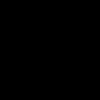
\includegraphics[width=0.38 \textwidth]{img/ex.png}
        \vspace{-5pt}
        \caption*{Caption here.}
        \vspace{-20pt}
        \label{fig:attitude-distribution}
    \end{wrapfigure}
    
\section{Data Retrieval}
\label{section:retrieval}

    f

\section{Data Processing}
\label{section:processing}

    d
    
\section{Analysis}
\label{section:analysis}

    d

\section{Conclusion}
\label{section:conclusion}

    d

\section{Critique}
\label{section:critique}

    d

\newpage

\onecolumn
\printbibliography[heading=bibintoc, title={References}]


\end{document}
